\documentclass[aspectratio=169]{beamer}

% ============================================================
% PACKAGES
% ============================================================
\usepackage{tikz}
\usetikzlibrary{calc, positioning, shapes.geometric}
\usepackage{tcolorbox}
\tcbuselibrary{skins, breakable}
\usepackage{fontawesome5}
\usepackage{amsmath, amssymb}
\usepackage{graphicx}
\usepackage{xcolor}
\usepackage{booktabs}
\usepackage{colortbl}
\usepackage{array}

% ============================================================
% COLOR PALETTE
% ============================================================
\definecolor{NavyBlue}{RGB}{8, 24, 58}
\definecolor{AccentBlue}{RGB}{0, 112, 200}
\definecolor{AccentCyan}{RGB}{0, 200, 210}
\definecolor{LightBg}{RGB}{244, 247, 253}
\definecolor{CardBg}{RGB}{255, 255, 255}
\definecolor{DarkCode}{RGB}{18, 22, 38}
\definecolor{CodeGreen}{RGB}{72, 199, 116}
\definecolor{CodeYellow}{RGB}{255, 198, 70}
\definecolor{CodeBlue}{RGB}{100, 180, 255}
\definecolor{CodePurple}{RGB}{200, 130, 255}
\definecolor{RowOdd}{RGB}{232, 241, 255}
\definecolor{RowEven}{RGB}{255, 255, 255}
\definecolor{HeaderRow}{RGB}{8, 24, 58}
\definecolor{SuccessGreen}{RGB}{0, 150, 100}
\definecolor{WarnOrange}{RGB}{240, 130, 30}

% ============================================================
% BEAMER THEME RESET
% ============================================================
\usetheme{default}
\usecolortheme{default}
\setbeamertemplate{navigation symbols}{}

% Background
\setbeamercolor{background canvas}{bg=LightBg}

% Fonts
\setbeamerfont{frametitle}{size=\large, series=\bfseries}
\setbeamerfont{title}{size=\LARGE, series=\bfseries}
\setbeamerfont{subtitle}{size=\normalsize, series=\mdseries}

% ============================================================
% FRAME TITLE
% ============================================================
\setbeamercolor{frametitle}{fg=white, bg=NavyBlue}
\setbeamertemplate{frametitle}{%
  \nointerlineskip%
  \begin{beamercolorbox}[wd=\paperwidth, ht=0.9cm, dp=0.15cm, leftskip=0.55cm]{frametitle}%
    \vbox to 0.9cm{\vfil\usebeamerfont{frametitle}\insertframetitle\vfil}%
  \end{beamercolorbox}%
  \nointerlineskip%
  {\color{AccentBlue}\hrule height 2.5pt}%
  \nointerlineskip%
}

% ============================================================
% FOOTER WITH PROGRESS BAR
% ============================================================
\setbeamercolor{footline bg}{bg=NavyBlue, fg=white}
\setbeamercolor{progress bar color}{bg=AccentCyan}

\setbeamertemplate{footline}{%
  \leavevmode%
  \begin{beamercolorbox}[wd=\paperwidth, ht=0.4cm, dp=0.15cm,
      leftskip=0.35cm, rightskip=0.35cm]{footline bg}%
    \tiny\color{white!70}AI-Integrated Washing Machine%
    \hfill%
    \color{white}\bfseries\insertframenumber\,/\,\inserttotalframenumber\hspace{0.1cm}%
  \end{beamercolorbox}%
  \vskip0pt%
}

% ============================================================
% BULLET STYLE
% ============================================================
\setbeamertemplate{itemize item}{\color{AccentBlue}\small\faAngleRight}
\setbeamertemplate{itemize subitem}{\color{AccentBlue!60}\scriptsize\faCircle}
\setbeamertemplate{enumerate item}{%
  \color{white}\footnotesize%
  \tikz[baseline=(n.base)]\node[fill=NavyBlue, circle, inner sep=1.8pt](n)%
    {\color{white}\tiny\bfseries\insertenumlabel};}

% ============================================================
% TCOLORBOX STYLES
% ============================================================
\tcbset{
  mycard/.style={
    enhanced, skin=enhancedmiddle jigsaw,
    colback=CardBg,
    colframe=NavyBlue,
    colbacktitle=NavyBlue,
    coltitle=white,
    fonttitle=\bfseries\small,
    boxrule=0.6pt,
    arc=5pt,
    left=5pt, right=5pt, top=4pt, bottom=4pt,
    toptitle=3pt, bottomtitle=3pt,
    drop fuzzy shadow={opacity=0.07, color=NavyBlue}
  },
  accentcard/.style={
    enhanced,
    colback=AccentBlue!7,
    colframe=AccentBlue,
    colbacktitle=AccentBlue,
    coltitle=white,
    fonttitle=\bfseries\small,
    boxrule=0.6pt,
    arc=5pt,
    left=5pt, right=5pt, top=4pt, bottom=4pt,
    toptitle=3pt, bottomtitle=3pt,
  },
  darkcode/.style={
    enhanced,
    colback=DarkCode,
    colframe=AccentBlue!80,
    coltitle=AccentCyan,
    colbacktitle=DarkCode!90,
    fonttitle=\bfseries\small\ttfamily,
    boxrule=0.8pt,
    arc=5pt,
    left=8pt, right=8pt, top=5pt, bottom=5pt,
    toptitle=3pt, bottomtitle=3pt,
    borderline north={1.5pt}{0pt}{AccentCyan!60},
  },
  successbox/.style={
    enhanced,
    colback=SuccessGreen!8,
    colframe=SuccessGreen,
    colbacktitle=SuccessGreen,
    coltitle=white,
    fonttitle=\bfseries\small,
    boxrule=0.6pt,
    arc=5pt,
    left=5pt, right=5pt, top=3pt, bottom=3pt,
    toptitle=3pt, bottomtitle=3pt,
  },
  infobar/.style={
    enhanced,
    colback=NavyBlue!5,
    colframe=NavyBlue!25,
    arc=4pt,
    boxrule=0.4pt,
    left=5pt, right=5pt, top=3pt, bottom=3pt,
  },
  goalbar/.style={
    enhanced,
    colback=AccentCyan!10,
    colframe=AccentCyan!70,
    arc=4pt,
    boxrule=0.5pt,
    left=5pt, right=5pt, top=3pt, bottom=3pt,
  },
}

% Helper command
\newcommand{\mybullet}{\textcolor{AccentBlue}{\small\faAngleRight}\;}

% ============================================================
% SECTION DIVIDERS — FULL BLEED
% ============================================================
\AtBeginSection[]{
  \begin{frame}[plain]
  \begin{tikzpicture}[remember picture, overlay]
    % Full background
    \fill[NavyBlue] (current page.south west) rectangle (current page.north east);

    % Left accent strip
    \fill[AccentBlue]
      ([xshift=1.3cm]current page.south west) rectangle
      ([xshift=1.65cm]current page.north west);
    \fill[AccentCyan]
      ([xshift=1.65cm]current page.south west) rectangle
      ([xshift=1.72cm]current page.north west);

    % Large ghost section number
    \node[text=AccentBlue!22, font=\fontsize{90}{90}\selectfont\bfseries,
          anchor=east] at ([xshift=-0.5cm]current page.east) {\thesection};

    % Section label
    \node[text=AccentCyan, font=\small\bfseries\sffamily, anchor=west]
      at ([xshift=2.1cm, yshift=1.0cm]current page.west) {SECTION \thesection};

    % Section title
    \node[text=white, font=\LARGE\bfseries, anchor=west, text width=11cm]
      at ([xshift=2.1cm, yshift=-0.1cm]current page.west) {\insertsectionhead};

    % Bottom thin accent line
    \fill[AccentCyan]
      ([yshift=0.45cm]current page.south west) rectangle
      ([xshift=5cm, yshift=0.52cm]current page.south west);
  \end{tikzpicture}
  \end{frame}
}

% ============================================================
% METADATA
% ============================================================
\title{AI-Integrated Fully Automatic Washing Machine}
\subtitle{Mini Project Presentation}
\author{
  Mihal Palakkal \quad Ruvais P \quad Mohamed Jaseeb P J \\
  Sajad Hussain Malla \quad Rishap Raj Chaudhary
}
\institute{%
  Department of Computer Science and Engineering\\
  \textbf{Cochin University of Science and Technology}\\[0.3cm]
  \textbf{Guide:} Ms.~Amrutha S~Nair\quad
  \textbf{Coordinator:} Dr.~Sheena~S%
}
\date{March 16, 2026}

% ============================================================
\begin{document}
% ============================================================

% ------------------------------------------------------------------
% TITLE SLIDE
% ------------------------------------------------------------------
\begin{frame}[plain]

\begin{tikzpicture}[remember picture, overlay]

  % --- Background ---
  \fill[NavyBlue] (current page.south west) rectangle (current page.north east);

  % --- Right panel ---
  \fill[NavyBlue!60]
    ([xshift=10.4cm]current page.south west) rectangle (current page.north east);
  \fill[AccentBlue]
    ([xshift=10.4cm]current page.south west) rectangle
    ([xshift=10.68cm]current page.north west);

  % --- Decorative circles (right panel) ---
  \fill[AccentBlue!30]
    ([xshift=13.7cm, yshift=4.8cm]current page.south west) circle (3.8cm);
  \fill[NavyBlue!80]
    ([xshift=13.7cm, yshift=4.8cm]current page.south west) circle (3.0cm);
  \node[text=AccentCyan, font=\fontsize{42}{50}\selectfont]
    at ([xshift=13.7cm, yshift=4.8cm]current page.south west) {\faRobot};

  % --- Title area ---
  \def\leftmargin{0.85cm}

  % Cyan accent bar
  \fill[AccentCyan]
    ([xshift=\leftmargin, yshift=3.7cm]current page.south west) rectangle
    ([xshift=\leftmargin+8.8cm, yshift=3.77cm]current page.south west);

  % Main title
  \node[anchor=south west, text=white, font=\fontsize{32}{36}\selectfont\bfseries,
        text width=9.5cm, inner sep=0pt]
    at ([xshift=\leftmargin, yshift=4.85cm]current page.south west)
    {AI-Integrated\\[2pt]Fully Automatic\\[4pt]Washing Machine};

  % Subtitle
  \node[anchor=north west, text=AccentCyan, font=\large\sffamily\bfseries,
        inner sep=0pt]
    at ([xshift=\leftmargin, yshift=4.3cm]current page.south west)
    {\faProjectDiagram\enspace Mini Project Presentation};

  % Authors
  \node[anchor=north west, text=white, font=\small,
        text width=9.5cm, inner sep=0pt]
    at ([xshift=\leftmargin, yshift=3.35cm]current page.south west)
    {%
      \textcolor{AccentCyan!80}{\textbullet}~\textbf{Mihal Palakkal}\quad
      \textcolor{AccentCyan!80}{\textbullet}~\textbf{Ruvais P}\quad
      \textcolor{AccentCyan!80}{\textbullet}~\textbf{Mohamed Jaseeb P J}\\[4pt]
      \textcolor{AccentCyan!80}{\textbullet}~\textbf{Sajad Hussain Malla}\quad
      \textcolor{AccentCyan!80}{\textbullet}~\textbf{Rishap Raj Chaudhary}%
    };

  % Institute + divider
  \draw[white!20, line width=0.5pt]
    ([xshift=\leftmargin, yshift=2.15cm]current page.south west) --
    ([xshift=\leftmargin+8.8cm, yshift=2.15cm]current page.south west);

  % Institute
  \node[anchor=north west, text=white!70, font=\scriptsize, text width=9.5cm,
        inner sep=0pt]
    at ([xshift=\leftmargin, yshift=2.05cm]current page.south west)
    {\faBuilding\enspace Dept.\ of Computer Science and Engineering\\
     \faGraduationCap\enspace \textbf{Cochin University of Science and Technology}};

  % Guide Section
  \node[anchor=north west, text=AccentCyan!80, font=\footnotesize, text width=9.5cm,
        inner sep=0pt]
    at ([xshift=\leftmargin, yshift=1.3cm]current page.south west)
    {\faUserTie\enspace \textbf{Guide:}\enspace Ms.\ Amrutha S Nair\hfill
     \faUserTie\enspace \textbf{Coordinator:}\enspace Dr.\ Sheena S};

  % Date (bottom-right)
  \node[anchor=south east, text=white!35, font=\tiny\sffamily]
    at ([xshift=-0.5cm, yshift=0.35cm]current page.south east) {March 16, 2026};

\end{tikzpicture}
\end{frame}

% ------------------------------------------------------------------
% OUTLINE
% ------------------------------------------------------------------
\begin{frame}{Outline}
\vspace{0.15cm}
\tableofcontents
\end{frame}

% ==================================================================
\section{Introduction}
% ==================================================================

\begin{frame}{Problem Statement \& Objective}
\begin{columns}[T]
\begin{column}{0.48\textwidth}
\begin{tcolorbox}[mycard,
  title={\faExclamationTriangle\enspace Problem}]
\small
Existing semi-automatic machines \textbf{waste water and detergent}, and damage clothes due to \textbf{fixed, non-adaptive} wash cycles.
\end{tcolorbox}
\end{column}
\begin{column}{0.48\textwidth}
\begin{tcolorbox}[accentcard,
  title={\faBullseye\enspace Objective}]
\small
Convert a semi-automatic machine into a \textbf{fully automated, AI-powered} system that:
\begin{itemize}
  \item Identifies cloth type via smartphone camera
  \item Optimizes wash parameters per fabric type
\end{itemize}
\end{tcolorbox}
\end{column}
\end{columns}
\vspace{0.35cm}
\begin{tcolorbox}[goalbar]
\centering\small
\textcolor{NavyBlue}{\faStar\enspace\textbf{Goal:}}
\emph{Intelligent washing that preserves fabric quality and conserves resources.}
\end{tcolorbox}
\end{frame}

% ------------------------------------------------------------------
\begin{frame}{System Architecture}

\begin{center}

\begin{tikzpicture}[
  box/.style={%
    rectangle, rounded corners=5pt,
    fill=NavyBlue, text=white,
    font=\small\bfseries,
    minimum height=0.78cm, minimum width=2.2cm,
    align=center, inner sep=5pt},
  arr/.style={->, thick, color=AccentBlue, >=stealth, line width=1.2pt}
]
\node[box] (img)     {Cloth\\[-1pt]\scriptsize Image};
\node[box, right=1.1cm of img]     (app)     {Mobile\\[-1pt]\scriptsize App};
\node[box, right=1.1cm of app]     (gemini)  {Gemini\\[-1pt]\scriptsize API};
\node[box, right=1.1cm of gemini]  (arduino) {Arduino\\[-1pt]\scriptsize WiFi R4};
\node[box, right=1.1cm of arduino] (machine) {Washing\\[-1pt]\scriptsize Machine};

\draw[arr] (img)     -- (app);
\draw[arr] (app)     -- (gemini);
\draw[arr] (gemini)  -- (arduino);
\draw[arr] (arduino) -- (machine);
\end{tikzpicture}
\end{center}

\vspace{0.25cm}
\textcolor{NavyBlue}{\textbf{Two-Stage AI Pipeline:}}
\vspace{0.18cm}

\begin{columns}[T]
\begin{column}{0.48\textwidth}
\begin{tcolorbox}[accentcard,
  title={\faSearch\enspace Stage 1: Fabric Detection}]
\small Identifies fabric type, fiber category, and soil level.
\end{tcolorbox}
\end{column}
\begin{column}{0.48\textwidth}
\begin{tcolorbox}[mycard,
  title={\faCogs\enspace Stage 2: Parameter Calculation}]
\small Computes optimal wash settings based on Stage 1 output.
\end{tcolorbox}
\end{column}
\end{columns}
\end{frame}

% ------------------------------------------------------------------
\begin{frame}{System Architecture Overview}
\centering\vspace{0.15cm}
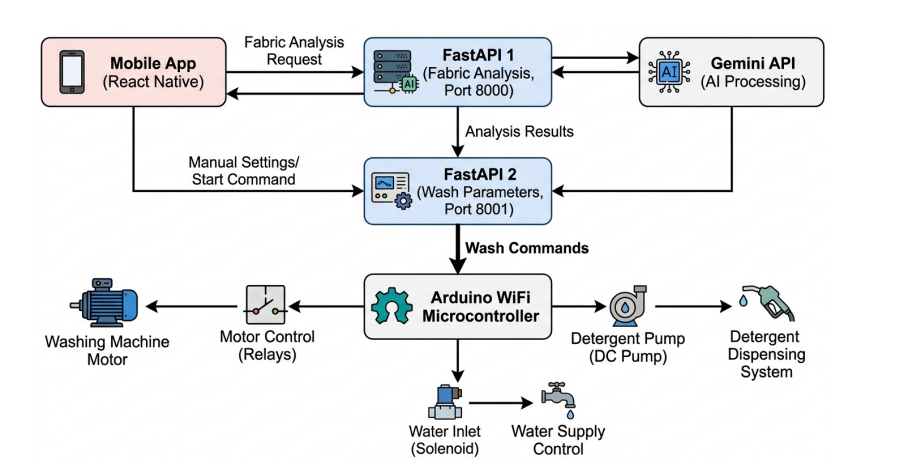
\includegraphics[width=0.9\textwidth, height=0.65\textheight,
  keepaspectratio]{img/system_overview.png}
\\[0.3cm]
{\small\textcolor{NavyBlue}{\faArrowRight\enspace\textbf{Flow:}}
  Image $\rightarrow$ Gemini (Stage 1 \& 2)
  $\rightarrow$ Arduino $\rightarrow$ Machine Actuation}
\end{frame}

% ==================================================================
\section{Hardware Design}
% ==================================================================

\begin{frame}{Hardware Components}
\begin{columns}[T]
\begin{column}{0.48\textwidth}
\begin{tcolorbox}[mycard,
  title={\faMicrochip\enspace Core \& Commutation}]
\small
\begin{itemize}
  \item Semi-automatic Washing Machine
  \item Arduino WiFi R4
  \item 3-Phase Motor (240V, 10A)
  \item 2 Rotation Relays + 1 Solenoid Relay
\end{itemize}
\end{tcolorbox}
\end{column}
\begin{column}{0.48\textwidth}
\begin{tcolorbox}[accentcard,
  title={\faWater\enspace Dispensing \& Actuation}]
\small
\begin{itemize}
  \item Solenoid Water Inlet Valve
  \item 5V DC Water Pump (Detergent)
  \item Transistor TAS122
  \item 12V L298N DC Motor Driver
\end{itemize}
\end{tcolorbox}
\end{column}
\end{columns}
\vspace{0.35cm}
\begin{tcolorbox}[infobar]
\centering\small
\textcolor{NavyBlue}{\faInfoCircle\enspace}
All components integrated to automate washing, dispensing, and motor control.
\end{tcolorbox}
\end{frame}

% ------------------------------------------------------------------
\begin{frame}{Hardware Design \& Control Logic}
\begin{columns}[T]
\begin{column}{0.60\textwidth}
\begin{itemize}
  \item \textbf{Motor Control:}
    Clockwise 5\,s $\rightarrow$ Stop 2\,s $\rightarrow$ Counter-clockwise 5\,s
    (loop) via relays.
  \item \textbf{Detergent Dispenser:} Linear regression calculates valve open time.
  \begin{itemize}
    \item Data collected at 50\,ms \dots\ 2400\,ms intervals.
    \item Regression equation implemented in Arduino code.
  \end{itemize}
  \item \textbf{Water Inlet Valve:} Same calibration approach for accurate filling.
\end{itemize}
\end{column}
\begin{column}{0.37\textwidth}
\begin{tcolorbox}[mycard, title={\faCalculator\enspace Regression Model}]
\centering\small
\[
  t \;=\; a \cdot V + b
\]
\scriptsize
$t$: open time (ms)\\
$V$: desired volume (ml)\\
$a,\,b$: calibration coefficients
\end{tcolorbox}
\end{column}
\end{columns}
\end{frame}

% ------------------------------------------------------------------
\begin{frame}{Detergent Dispenser Calibration}
\begin{columns}[T]
\begin{column}{0.50\textwidth}
\begin{tcolorbox}[mycard, title={\faTable\enspace Calibration Data}]
\centering\scriptsize\setlength{\tabcolsep}{3.5pt}
\rowcolors{2}{RowOdd}{RowEven}
\begin{tabular}{cc|cc|cc}
\rowcolor{HeaderRow}
\color{white}\textbf{ms} & \color{white}\textbf{ml} &
\color{white}\textbf{ms} & \color{white}\textbf{ml} &
\color{white}\textbf{ms} & \color{white}\textbf{ml}\\
 50 & 0.0  & 650  & 10.25 & 1400 & 26.5 \\
100 & 0.0  & 700  & 11.5  & 1500 & 28.0 \\
150 & 0.0  & 750  & 12.0  & 1600 & 30.0 \\
200 & 0.5  & 800  & 13.0  & 1700 & 33.0 \\
250 & 2.0  & 850  & 15.0  & 1800 & 35.5 \\
300 & 3.0  & 900  & 16.5  & 1900 & 39.5 \\
350 & 4.5  & 950  & 18.0  & 2000 & 41.5 \\
400 & 5.0  &1000  & 19.0  & 2100 & 44.5 \\
450 & 6.0  &1050  & 20.0  & 2200 & 46.0 \\
500 & 7.5  &1100  & 21.0  & 2300 & 48.0 \\
550 & 8.5  &1200  & 23.0  & 2400 & 50.5 \\
600 & 9.75 &1300  & 25.5  & ---  & ---  \\
\end{tabular}
\end{tcolorbox}
\end{column}
\begin{column}{0.47\textwidth}
\begin{tcolorbox}[accentcard, title={\faChartLine\enspace Linear Regression}]
\centering
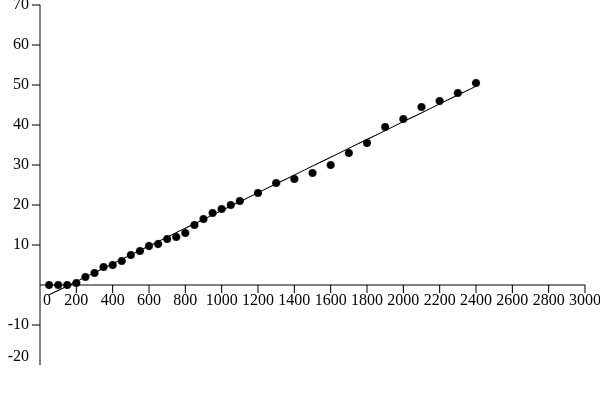
\includegraphics[width=0.92\textwidth, height=0.30\textheight,
  keepaspectratio]{img/graph.png}
\end{tcolorbox}

\vspace{0.22cm}
\begin{tcolorbox}[mycard, title={\faCalculator\enspace Model Coefficients}]
\centering\small\setlength{\tabcolsep}{5pt}
\rowcolors{2}{RowOdd}{RowEven}
\begin{tabular}{lc}
\rowcolor{HeaderRow}
\color{white}\textbf{Coefficient} & \color{white}\textbf{Value}\\
$a$ (slope)     & 0.022176   \\
$b$ (intercept) & $-$3.569687\\
$R^2$ value     & 0.997      \\
\end{tabular}
\end{tcolorbox}
\end{column}
\end{columns}
\end{frame}

% ==================================================================
\section{AI \& Backend}
% ==================================================================

\begin{frame}{Fabric Analysis — Stage 1 (Gemini API)}
\begin{columns}[T]
\begin{column}{0.50\textwidth}
\begin{tcolorbox}[mycard, title={\faBrain\enspace Multi-Stage Prompt System}]
\small Extracts the following from a cloth image:
\begin{itemize}
  \item Fabric name
  \item Fiber category
  \item Soil level (1–5 scale)
\end{itemize}
\vspace{0.18cm}
\textbf{Visual markers analyzed:}\\
\textcolor{AccentBlue!80}{\small diagonal ribbing, fiber luster, fold behavior.}
\end{tcolorbox}
\end{column}
\begin{column}{0.46\textwidth}
\begin{tcolorbox}[accentcard, title={\faThermometerHalf\enspace Soil Level Scale}]
\small
\begin{tabular}{@{}cl@{}}
\textcolor{SuccessGreen}{\textbf{1}} & Clean \\[3pt]
\textcolor{AccentBlue}{\textbf{2}}   & Lightly Soiled \\[3pt]
\textcolor{CodeYellow}{\textbf{3}}   & Moderately Dirty \\[3pt]
\textcolor{WarnOrange}{\textbf{4}}   & Heavily Soiled \\[3pt]
\textcolor{red!80}{\textbf{5}}       & Emergency \\
\end{tabular}
\end{tcolorbox}
\end{column}
\end{columns}
\end{frame}

% ------------------------------------------------------------------
\begin{frame}{Stage 1 — JSON Output}
\begin{tcolorbox}[darkcode,
  title={\faCode\enspace Output JSON — Stage 1: Fabric Analysis}]
\color{white}\ttfamily\small
\{\\[2pt]
\quad\textcolor{CodeYellow}{"material\_type"}\,:\,\textcolor{CodeGreen}{"cotton twill"},\\[2pt]
\quad\textcolor{CodeYellow}{"fiber\_category"}\,:\,\textcolor{CodeGreen}{"Natural"},\\[2pt]
\quad\textcolor{CodeYellow}{"description"}\,:\,\textcolor{CodeGreen}{"Heavy cotton fabric with diagonal ribs"},\\[2pt]
\quad\textcolor{CodeYellow}{"dirt\_level"}\,:\,\textcolor{CodePurple}{3},\\[2pt]
\quad\textcolor{CodeYellow}{"confidence\_score"}\,:\,\textcolor{CodePurple}{0.92}\\[2pt]
\}
\end{tcolorbox}
\end{frame}

% ------------------------------------------------------------------
\begin{frame}{Wash Parameter Calculation — Stage 2}
\vspace{0.05cm}
\small Takes JSON from Stage 1 and computes optimal wash settings:
\vspace{0.25cm}

\begin{columns}[T]
\begin{column}{0.48\textwidth}
\begin{tcolorbox}[mycard, title={\faFlask\enspace Wash Parameters}]
\small
\begin{itemize}
  \item Detergent: baseline 20\,ml, adjusted
  \item Soak: 0–30\,min
  \item Spin: 3–12\,min (fabric-based)
  \item Water: standard 35\,L
\end{itemize}
\end{tcolorbox}
\end{column}
\begin{column}{0.48\textwidth}
\begin{tcolorbox}[accentcard, title={\faSlidersH\enspace Cycle Controls}]
\small
\begin{itemize}
  \item Wash Cycles: 1–2
  \item Temperature: up to 60\,°C
  \item Action: Gentle / Normal / Heavy
\end{itemize}
\end{tcolorbox}
\end{column}
\end{columns}
\end{frame}

% ------------------------------------------------------------------
\begin{frame}{Stage 2 — JSON Output}
\begin{tcolorbox}[darkcode,
  title={\faCode\enspace Output JSON — Stage 2: Wash Parameters}]
\color{white}\ttfamily\small
\{\\[2pt]
\quad\textcolor{CodeYellow}{"detergent\_ml"}\,:\,\textcolor{CodePurple}{28},\\[2pt]
\quad\textcolor{CodeYellow}{"soak\_minutes"}\,:\,\textcolor{CodePurple}{15},\\[2pt]
\quad\textcolor{CodeYellow}{"spin\_minutes"}\,:\,\textcolor{CodePurple}{8},\\[2pt]
\quad\textcolor{CodeYellow}{"water\_liters"}\,:\,\textcolor{CodePurple}{35},\\[2pt]
\quad\textcolor{CodeYellow}{"wash\_cycles"}\,:\,\textcolor{CodePurple}{2},\\[2pt]
\quad\textcolor{CodeYellow}{"temperature\_c"}\,:\,\textcolor{CodePurple}{45},\\[2pt]
\quad\textcolor{CodeYellow}{"mechanical\_action"}\,:\,\textcolor{CodeGreen}{"Normal"}\\[2pt]
\}
\end{tcolorbox}
\end{frame}

% ------------------------------------------------------------------
\begin{frame}{FastAPI Backend}
\textcolor{NavyBlue}{\textbf{Two independent microservices:}}
\vspace{0.25cm}

\begin{columns}[T]
\begin{column}{0.48\textwidth}
\begin{tcolorbox}[mycard, title={\faServer\enspace API 1 — Fabric Analysis \small(Port 8000)}]
\small
\begin{itemize}
  \item Input: Cloth image
  \item Uses Pillow + Gemini API
  \item Predicts: fiber type, dirt level, description
  \item \textbf{Human-in-the-Loop} feedback for corrections
\end{itemize}
\end{tcolorbox}
\end{column}
\begin{column}{0.48\textwidth}
\begin{tcolorbox}[accentcard, title={\faServer\enspace API 2 — Wash Parameter Calculator}]
\small
\begin{itemize}
  \item Input: Stage 1 JSON
  \item Outputs optimized wash settings
  \item Direct serial I/O with Arduino
\end{itemize}
\end{tcolorbox}
\end{column}
\end{columns}
\vspace{0.28cm}
\begin{tcolorbox}[infobar]
\centering\small
\textbf{\textcolor{NavyBlue}{\faCode\enspace Tech Stack:}}
Python,\ FastAPI,\ Pydantic,\ Pillow,\ Gemini API,\ OpenAPI
\end{tcolorbox}
\end{frame}

% ==================================================================
\section{Mobile App \& Testing}
% ==================================================================

\begin{frame}{Mobile App (React Native Expo)}
\begin{columns}[T]
\begin{column}{0.34\textwidth}
\begin{tcolorbox}[mycard, title={\faMobile*\enspace 5 Screens}]
\small
\begin{enumerate}
  \item Dashboard
  \item Fabric Analysis
  \item Wash Progress
  \item Manual Override
  \item Settings
\end{enumerate}
\end{tcolorbox}
\end{column}
\begin{column}{0.62\textwidth}
\begin{tcolorbox}[accentcard, title={\faStar\enspace Key Features}]
\small
\begin{itemize}
  \item Reusable UI components (Step Indicators, Cards)
  \item TypeScript interfaces for data integrity
    \textit{\scriptsize (Fabric, MachineMetrics, CycleState)}
  \item Tailwind CSS utility-first styling
  \item Async API service layer connecting to backend
  \item Cross-platform (iOS \& Android)
\end{itemize}
\end{tcolorbox}
\vspace{0.2cm}
\begin{tcolorbox}[infobar]
\centering\small\textcolor{NavyBlue}{\faLink\enspace}
App communicates with FastAPI backends via REST calls.
\end{tcolorbox}
\end{column}
\end{columns}
\end{frame}

% ------------------------------------------------------------------
\begin{frame}{Mobile App Screenshots (1/2)}
\centering\vfill
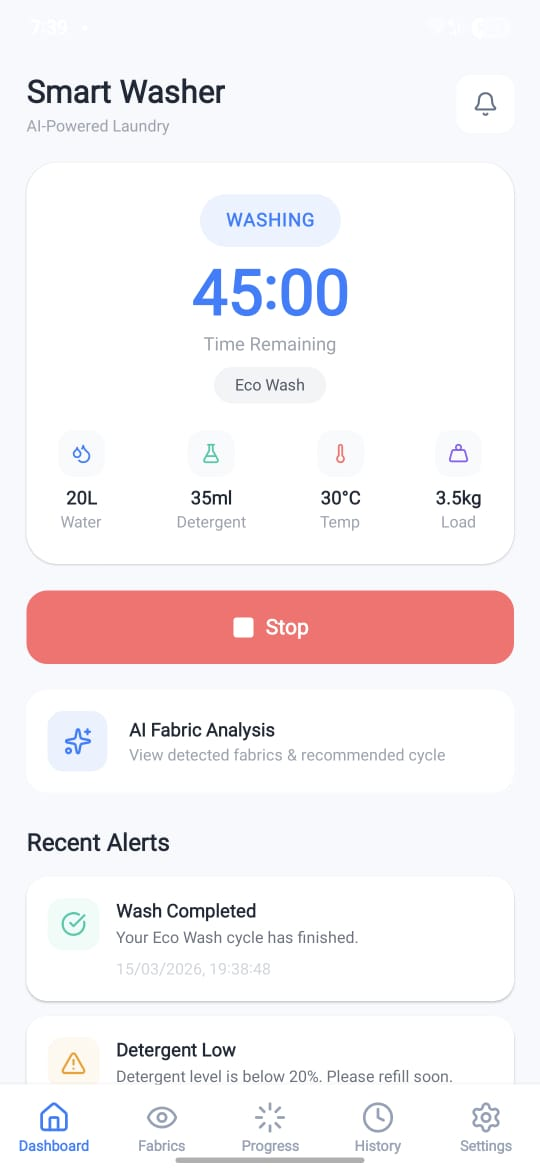
\includegraphics[height=0.65\textheight, keepaspectratio]{img/app1.jpeg}\hfill
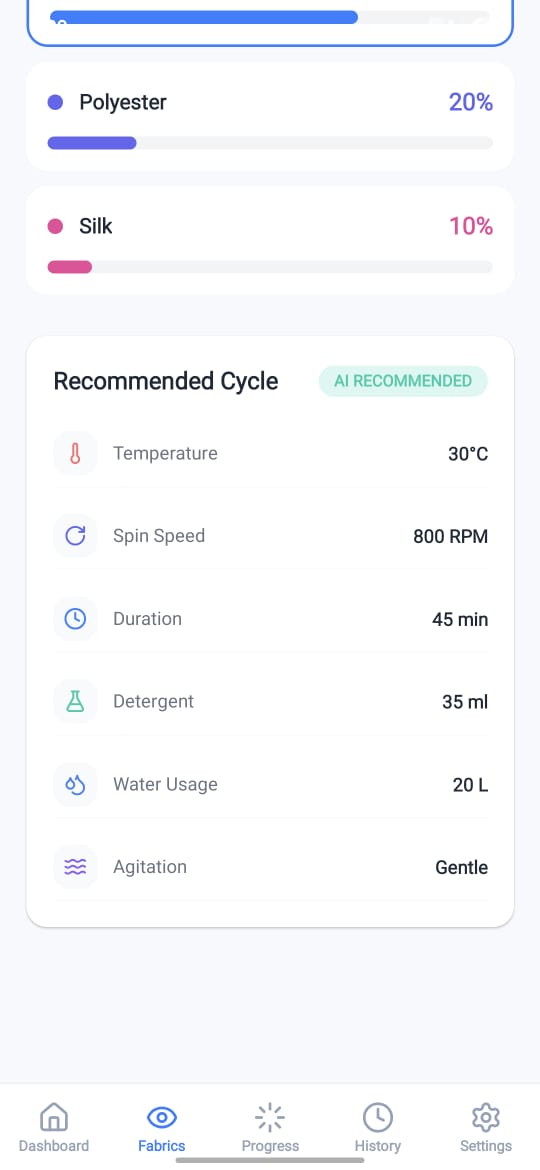
\includegraphics[height=0.65\textheight, keepaspectratio]{img/app2.jpeg}\hfill
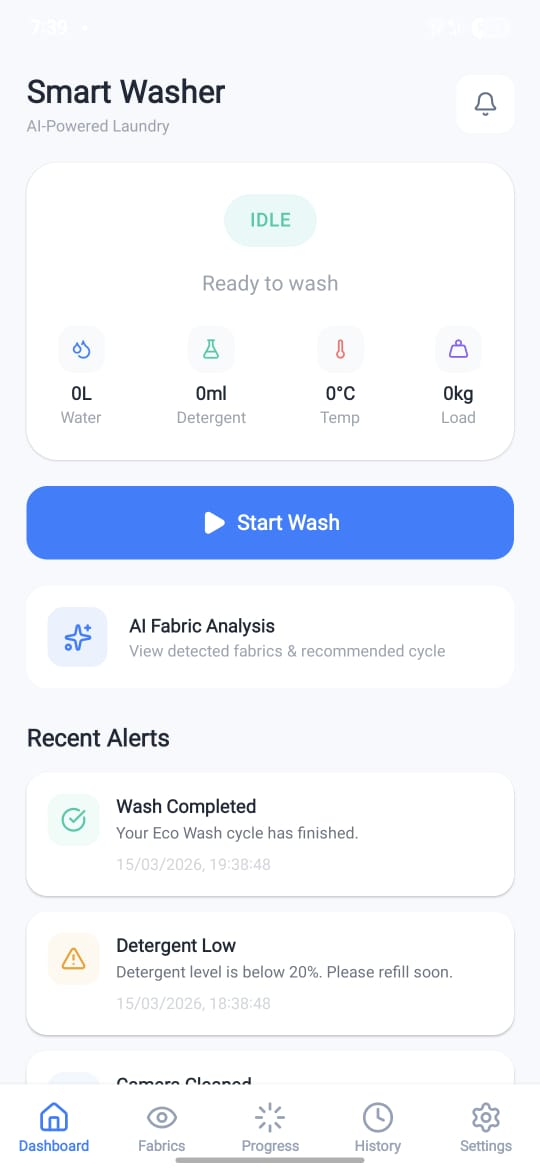
\includegraphics[height=0.65\textheight, keepaspectratio]{img/app3.jpeg}\hfill
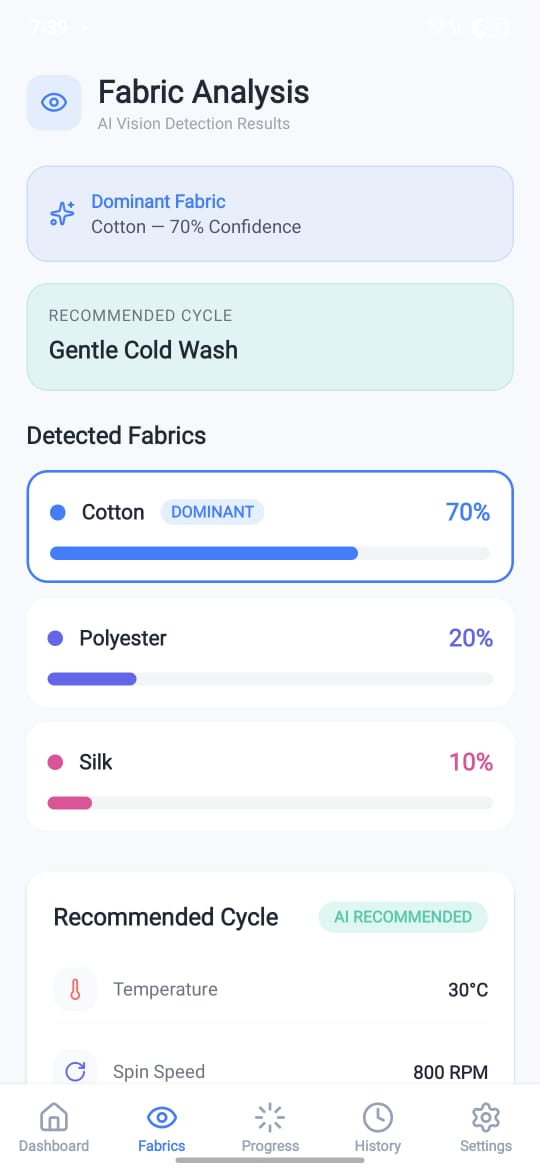
\includegraphics[height=0.65\textheight, keepaspectratio]{img/app4.jpeg}
\vfill
\end{frame}

% ------------------------------------------------------------------
\begin{frame}{Mobile App Screenshots (2/2)}
\centering\vfill

\includegraphics[height=0.65\textheight, keepaspectratio]{img/app5.jpeg}\hspace{0.5cm}
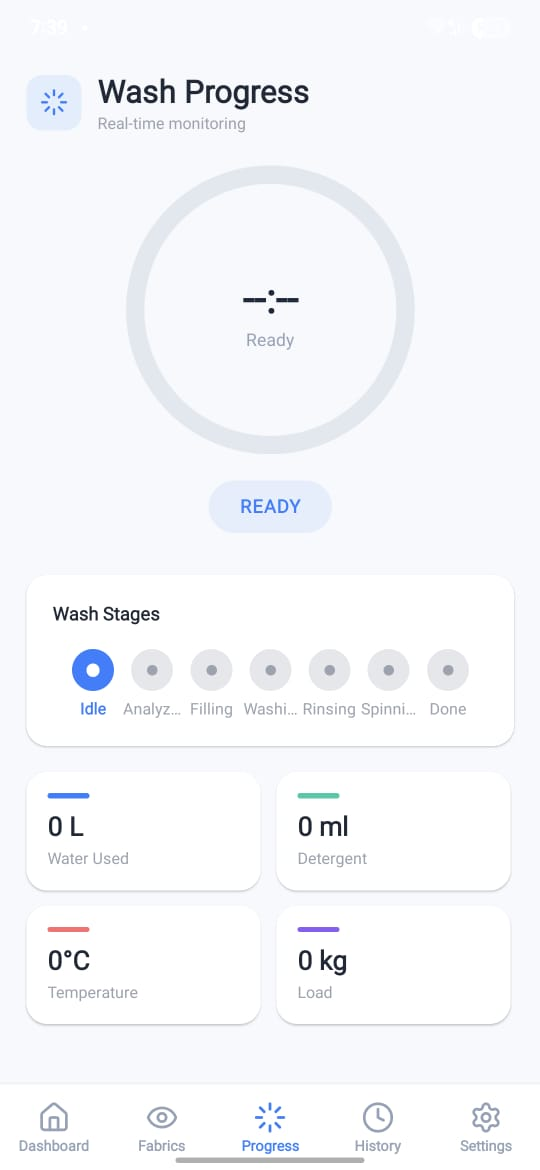
\includegraphics[height=0.65\textheight, keepaspectratio]{img/app6.jpeg}\hspace{0.5cm}
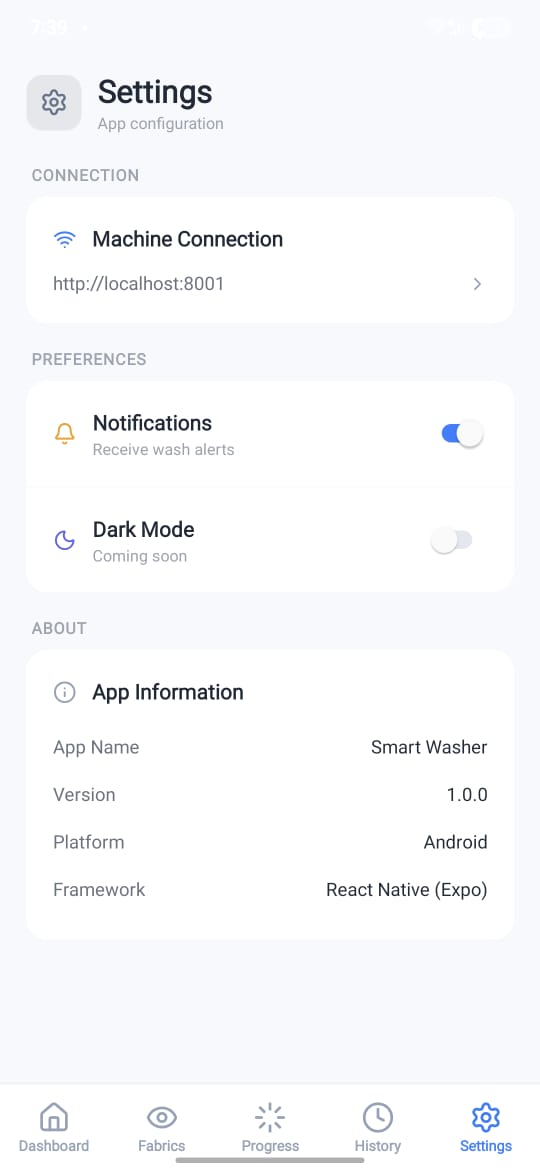
\includegraphics[height=0.65\textheight, keepaspectratio]{img/app7.jpeg}
\vfill
\end{frame}

% ------------------------------------------------------------------
\begin{frame}{Dataset Validation \& Testing}
\begin{itemize}
  \item Test cases from \textbf{heavy-duty (Denim)} to \textbf{delicate (Chiffon)}.
  \item \textbf{Human-in-the-Loop (HITL)} testing for misclassifications:
  \begin{itemize}
    \item Example: Differentiating \emph{Cotton Twill} vs \emph{Synthetic Blends}
    \item Iterative prompt refinement eliminated identification errors.
  \end{itemize}
  \item Standardized JSON output ensures seamless hardware integration.
  \item Detergent dispensing validated via linear regression (error $<5\%$).
\end{itemize}
\vspace{0.3cm}
\begin{tcolorbox}[successbox, title={\faCheckCircle\enspace Result}]
\centering
Reliable classification across \textbf{15+ fabric types} with high confidence scores.
\end{tcolorbox}
\end{frame}

% ==================================================================
\section{Results \& Future Scope}
% ==================================================================

\begin{frame}{Results \& Key Achievements}
\begin{itemize}
  \item \textbf{Accurate Fabric Classification:}
    High confidence scores across multiple fabric types.
  \item \textbf{Precise Detergent Dispensing:}
    Linear regression validated against real-world measurements.
  \item \textbf{End-to-End Automation:}
    Image scan $\rightarrow$ AI decision $\rightarrow$ Hardware execution.
  \item \textbf{Increased Cloth Lifetime:}
    Optimized parameters per fabric type reduce wear and tear.
  \item \textbf{Fully Functional Dual-API System:}
    Real-time feedback loop for continuous improvement.
\end{itemize}
\vspace{0.28cm}
\begin{tcolorbox}[successbox, title={\faTrophy\enspace Success}]
\centering
Successfully converted a semi-automatic machine into an
\textbf{intelligent, adaptive} washing system.
\end{tcolorbox}
\end{frame}

% ------------------------------------------------------------------
\begin{frame}{Conclusion \& Future Scope}
\begin{columns}[T]
\begin{column}{0.48\textwidth}
\begin{tcolorbox}[mycard, title={\faFlagCheckered\enspace Conclusion}]
\small
\begin{itemize}
  \item Demonstrated a \textbf{low-cost} AI-integrated laundry automation system.
  \item Bridges computer vision, prompt engineering, embedded systems, and mobile development.
\end{itemize}
\end{tcolorbox}
\end{column}
\begin{column}{0.48\textwidth}
\begin{tcolorbox}[accentcard, title={\faRocket\enspace Future Scope}]
\small
\begin{itemize}
  \item Weight sensor for load-based optimization.
  \item Cloud dashboard for wash history analytics.
  \item Multi-cloth batch scanning support.
  \item Smart home integration (Google Home, Alexa).
\end{itemize}
\end{tcolorbox}
\end{column}
\end{columns}
\end{frame}

% ------------------------------------------------------------------
% THANK YOU SLIDE
% ------------------------------------------------------------------
\begin{frame}[plain]
\begin{tikzpicture}[remember picture, overlay]

  \fill[NavyBlue] (current page.south west) rectangle (current page.north east);

  % Outer glow circle
  \fill[AccentBlue!25] (current page.center) circle (3.8cm);
  % Inner ring
  \fill[NavyBlue] (current page.center) circle (3.2cm);
  % Accent ring
  \draw[AccentCyan, line width=2pt] (current page.center) circle (3.2cm);

  % Text
  \node[text=white, font=\Huge\bfseries] at (current page.center) {Thank You!};

  \node[text=AccentCyan, font=\large]
    at ([yshift=-0.9cm]current page.center) {Questions?};

  \node[text=white!55, font=\small]
    at ([yshift=-1.65cm]current page.center) {\emph{We welcome your feedback.}};

  % Bottom credit
  \node[text=AccentBlue!60, font=\tiny]
    at ([yshift=0.35cm]current page.south)
    {AI-Integrated Fully Automatic Washing Machine \textbullet{} CUSAT \textbullet{} March 16, 2026};

\end{tikzpicture}
\end{frame}

\end{document}
